\section{Konzeption}

Nachfolgend soll nun zunächst die aktuelle Produktiv- und die aktuellen Testumgebungen beschrieben werden. Anschließend soll ein neuer Ansatz für eine Testumgebung auf Basis einer Virtualisierung definiert werden, mit dessen Hilfe sich später eine konkrete Implementierung umsetzen lässt. Zudem sollen die eingangs in der Problemstellung angedeuteten Probleme aufgrund fehlender isolierter Testumgebungen bei der Ausführung von Tests genauer erläutert und durch die Definition eines entsprechenden Beispieltests dargestellt werden. Dieser Test soll auch als Grundlage für eine Evaluierung der konkreten Implementierungen in Bezug auf ihre Ausführungsdauer dienen.

\subsection{Beschreibung der aktuellen Produktivumgebung}

Die Betriebsumgebung, die von der Pixelhouse GmbH in Produktion eingesetzt wird, besteht aus einer Vielzahl von Komponenten und Diensten. Diese Komponenten werden bislang jeweils auf echter Serverhardware betrieben.

\begin{figure}[!ht]
  \begin{center}
    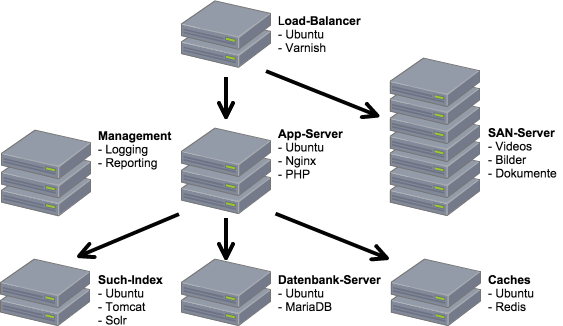
\includegraphics[width=10cm]{bilder/Produktiv-Umgebung.png}
    \caption{Die Produktiv-Umgebung der Webseite chefkoch.de}
  \end{center}
\end{figure}

Im Zentrum der Infrastruktur stehen insgesamt drei Appserver. Bei jedem Appserver handelt es sich dabei um einen Ubuntu-Server, auf dem der Webserver Nginx und der Script-Interpreter PHP ausgeführt wird, um HTTP-Anfragen mit Hilfe statischer oder dynamische Inhalte zu beantworten. Auf den App-Servern läuft somit auch die in PHP geschriebene Anwendung selbst. Für die langfristige Datenhaltung greifen die PHP-Scripte dabei auf zwei Datenbankserver (Master und Slave) zu, auf denen ebenfalls Ubuntu und der Mysql-Fork MariaDB installiert sind. Für kurzfristige und hochverfügbare Datencaches gibt es zwei Ubuntu-Server (Master und Slave) auf denen der Key-Value-Store Redis läuft. Zudem wird auf weiteren zwei Ubuntu-Servern (Master und Slave) ein Such-Index mit Hilfe der Suchmaschine Solr betrieben, die als Java-Anwendung in einem Tomcat-Application-Server läuft. Binärdateien (Videos, Bilder, Dokumente, etc.) werden auf insgesamt 7 weiteren Servern redundant abgelegt. Damit die Appserver und die SAN-Server von außen unter einheitlichen HTTP-Adressen erreichbar sind und sich die Last gleichmäßig auf die einzelnen Server verteilt, landen sämtliche HTTP-Anfragen per DNS-Round-Robin zunächst bei einem von zwei Ubuntu-Servern, auf denen Varnish als Load-Balancer installiert ist. Diese nehmen die Anfragen entgegen und verteilen sie an die dahinter liegenden Server. Varnish ist zudem ein effizienter HTTP-Cache, der in der Lage ist, die von den App- oder SAN-Servern zurückgelieferten Antworten zu cachen und bei erneuter Anfrage selbst auszuliefern. Zu guter Letzt gibt es noch drei weitere Server, auf denen Software für die Administration und das Reporting läuft.

\subsection{Beschreibung der aktuellen Testumgebung}

Die aktuellen Testumgebungen der Pixelhouse GmbH besitzen einen extrem reduzierten Aufbau. Die Testumgebungen werden alle auf ein und derselben Hardware-Maschine installiert. Fast alle Komponenten der zuvor beschriebenen Produktiv-Umgebung werden dabei von den einzelnen Testumgebungen gemeinsam verwendet. Beispielsweise nutzen alle Testumgebungen den gleichen Varnish für Load-Balancing und Caching. Dieser reicht die HTTP-Anfragen an den selben Nginx-Web-Server und PHP-Interpreter weiter und cached die Antworten bei Bedarf gleichermaßen. Als Backend-Dienste werden dieselbe MariaDB-Datenbank, derselbe Redis-Cache und derselbe Solr-Such-Index verwendet. Die Binärdateien werden ebenfalls auf demselben Host von allen Testumgebungen gemeinsam verwendet. Einziger Unterschied zwischen den einzelnen Testumgebungen ist, dass aufgrund einer speziellen Konfiguration im Nginx-Webserver je nach aufgerufener URL vom PHP-Interpreter andere PHP-Scripte geladen werden und somit jeweils eine andere Version der PHP-Anwendung getestet werden kann.

\begin{figure}[!ht]
  \begin{center}
    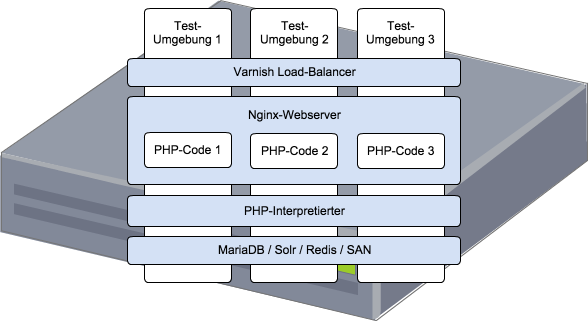
\includegraphics[width=10cm]{bilder/Aktuelle-Testumgebung.png}
    \caption{Die aktuelle Test-Umgebung}
  \end{center}
\end{figure}

Die aktuelle Testumgebung bringt Probleme in Bezug auf die Testbarkeit der Anwendung mit sich. Da alle Testumgebungen zum Beispiel die gleichen Backend-Dienste verwenden, ist es mitunter nicht möglich, die für den Test notwendigen Testdaten zu erzeugen, ohne damit Einfluss auf andere Testumgebungen zu nehmen. Ein weiteres Problem ist, dass nur Änderungen am PHP-Code selbst testbar sind. Will man zum Beispiel eine Änderung am HTTP-Caching im Varnish testen, kann man diese nur in allen Testumgebungen gleichermaßen vornehmen.

\subsection{Definition einer verifizierbaren Testumgebung}

Ziel der neuen Testumgebung muss es sein, einen der Produktivumgebung entsprechenden Aufbau zu besitzen. So sollen alle in Produktion vorhandenen Komponenten mit Hilfe der Virtualisierung als eigenständige Maschinen dargestellt werden, auch wenn sie tatsächlich auf nur einer echten Hardware-Maschine laufen. Es muss außerdem möglich sein, mehrere dieser Testumgebungen parallel zu betreiben.

\begin{figure}[!ht]
  \begin{center}
    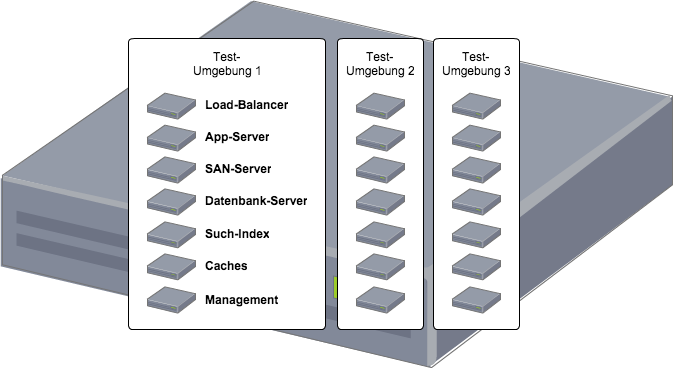
\includegraphics[width=10cm]{bilder/Untersuchungs-Umgebung.png}
    \caption{Für die Untersuchung definierte Umgebung}
  \end{center}
\end{figure}

Tests, die gegen eine solche virtuelle Testumgebung gestartet werden, dürfen sich dabei nicht gegenseitig beinflussen. Das Aufsetzen und Entfernen einer Testumgebung muss programmatisch und mit überschaubarem Zeitaufwand möglich sein. Die tatsächliche Konfiguration der einzelnen Komponenten der Umgebung sollte dabei selbst unter Versionskontrolle gestellt werden können, um langfristig Änderungen an der Infrastruktur nachvollziehen zu können. "`The change should be made to version control and then applied through your automated process for deploying infrastructural changes."' \citep[S.][S. 287]{HumFar10}

\subsection{Definition eines Testfalls}

TODO

\subsection{Verwendete Virtualisierungslösungen}

Im Folgenden sollen nun zwei konkrete Lösungen zur Erzeugung von Test- bzw. Betriebsumgebungen skizziert werden. Die konkret verwendeten Virtualisierungslösungen werden dabei von der Pixelhouse GmbH vorgegeben.

Zum einen setzt die Pixelhouse GmbH bereits Oracles VirtualBox ein, um eine lokale Entwicklungsumgebung für die Anwendung der Webseite chefkoch.de auf den Laptops der Entwickler vorzuhalten. VirtualBox ist somit bereits auf fast allen Rechnern vorhanden und es existieren grundlegende Kenntnisse und Erfahrungen für dieses Produkt.

Zum anderen wird aktuell von Seiten der Server-Administratoren das Produkt Docker eingeführt, um die Produktivumgebung der Plattform zu betreiben. Diverse Produktiv-Komponenten der Webseite chefkoch.de laufen also bereits innerhalb von Linux-Containern. Die ersten Erfahrungen der Administratoren sind dabei vielversprechend. Es besteht der Wunsch, Probleme zu minimieren, die auftreten, weil Entwicklungs-, Test- und Produktivumgebungen nicht die gleiche Technologie verwenden und sich so grundlegend voneinander unterscheiden.
